\chapter{Understanding}

\begin{quote}
 We can understand ... with a little common sense, without any miraculous insight specific to genius.
\attrib{George Pólya}
\end{quote}

\section{Perspective Collection}

\begin{quote}
You don't understand anything until you learn it more than one way.
\attrib{Marvin Minsky}
\end{quote}

I know a bit of abstract algebra, and I'm a decent cook. \marginnote{Cooking
has gotten me a lot more attention from women than abstract algebra ever has.}

The two subjects have a lot in common. And I don't mean this in some
maybe-deep-but-probably-not sense of, ``the reality of a fresh bagel is contained in mathematics and mathematics
is contained in a fresh bagel.'' I mean, sure, maybe symmetrical
recipes taste better.\footnote{Group theory, a subdomain of abstract algebra, is
  sometimes called the mathematics of symmetries, because groups can be used to
  describe (capture?) symmetries.} I don't know.

You'll need a better mathematician than me to speak about that.

No, what I mean is that learning either of these subjects can teach you the same
lesson about human cognition.

That lesson? \textbf{Like an entomologist during a killing jar 75\%-off sale, collect
  multiple specimens.}

When I want to cook something, I never read just one recipe\marginnote{Full
  disclosure: this is a lie. Sometimes I read just one recipe.} -- I read three
or five or thirteen.

With so many recipes, you can use your pattern matching bazooka. Ask yourself, ``What's
constant across all of these?'' And once you know the answer to that,
you've figured out the quintessence of a dish.

Wittgenstein can argue all he wants about the definition of a
game\footnote{``The problem is that there is no property common to all games, so that the most usual kinds of definition fail.''} but, read 5
recipes for the same thing, and you'll have a definition of that dish. And you
don't even need some platonic cookbook sent down from on high. Just an internet
connection.

Understand the essence of pineapple fried rice and, like Charlie Parker,\marginnote{Charlie
  Parker was a jazz giant and improv king.} you're free to improvise. And that's what cooking is about. Grasping the underlying pieces of a recipe
that make it \textit{it} and then adding your twist to it. A delicious
cinnamon-sriracha-peanut-butter twist.

\newthought{To understand} abstract algebra, use the same method. If you want to know what a field,
or a group, or a monoid is, you can't read one recipe, one treatment. You need
to read three or seventeen. Flip through thirteen textbooks. Decipher those and
you'll dream about algebraic fields. Nasty, R-rated dreams, where a
\textit{fuh-ine} field rings the doorbell, pizza-delivery in hand, and, well, you know.

\newthought{Or consider} mathematical proof.

What's the point of knowing multiple proofs for the same theorem? Once something
has been proven, why do mathematicians continue searching for cleaner, more
elegant proofs?

It's proved. It's valid. The matter has been settled. The thing is done! Shadows
of doubt no more, \textit{we can walk in the open air.} Proof, sir! Proof.

But more? \textit{Another?} You wouldn't imprison two men for the same crime.

\newthought{Okay, alright.} You've caught me: the purpose of multiple proof, and even proof in
general, is insight. The purpose is \textit{not} to to erect perfect logical
towers of eternal truth, immune to all criticism.

Seen this way, of course we want multiple proofs, just as we want multiple
recipes: each, if we're lucky, sheds some additional light on the structure. Our mental
picture becomes sharper, more defined.

We start to feel that we know.

\newthought{So we've} generalized this method from recipes, to abstract algebra, to math and proofs
as a whole, but don't stop there: \textbf{to understand anything, anything at all, in
  any significant way, collect multiple perspectives. Be that killing-jar-happy
  entomologist.}

5, 7, 13. The number of perspectives you need varies. Simple subject? Maybe just
one. Complex? I can (very scientifically) assure you that between 83 and 87
examples should be enough.

\newthought{This idea} is so powerful that it's not limited to humans. Hell, it's
not even limited to organic life. There have been some advances in
automated theorem proving by training programs on several different proofs of
the same theorem -- exactly the idea I've just told you about. (See, for
instance, \href{http://intelligence.org/2013/12/21/josef-urban-on-machine-learning-and-automated-reasoning/}{this interview}.)

% tk find link/citation

\section{Debugging Confusion}
\begin{quote}
A person taking a test or playing a piece of music is executing a program, a
deterministic procedure.  If your program has a bug, then you'll get a whole
class of problems wrong, consistently.
\attrib{celandine13, \href{http://celandine13.livejournal.com/33599.html}{the most insightful LiveJournal entry of all time}}
\end{quote}

Lend me your imagination for a minute.

One day, you're cleaning your attic. Light filters in through some crooked
blinds. It highlights the (significant) dust in the air, and you can make out
each speck, like a tiny alien race, come to colonize your attic. 

It's hot. You wonder why you volunteered for this project in the first place.

You're emptying a chest of drawers and you stumble across... well, it's what
looks like a glass sphere -- sorta a snow globe, but sans base.

It has to be old, given the amount of grime that it's accumulated. The muck
coats your fingers. Your nose curls and you grimace in a moment of disgust, and then you grab a
towel -- first each finger, and then you polish off the mutant snow
globe.

And, as it starts to gleam, your attention latches onto the tiny glass planet,
until, with a start, you realize that you can't feel your body. It's like your
consciousness has been possessed, and you can't steal your eyes away from the
ball.

Bit by bit, the attic around you disappears like television static, and you find your awareness floating,
bodyless, over a boy hunched over a math problem set and a sheet of paper. He
grips a pencil and, by his side, there lies the nub of what used to be a meaty
eraser.

As he flips through the back of the calculus book, the look of concentration on
his face is replaced with one of expectation. He lands on a page. 

His fist strikes the table.

There's a frustrated bellow-grunt, and you hear him say, "I'm too stupid. I'll
never get this."

You, too, are swept away in a moment of shared frustration, as your mind is
doubly hijacked: first by the snow globe, and now by empathy.

You wonder why the ball has sent you here, to this particular time and place,
and then...

\section{What's in a skill? }

Here's something I dislike: when people describe something as algorithmic as an
insult. Oh, \textit{that}, it's so algorithmic. A computer could do that.

Like when colleges tout that oh, well, we have humans review each child's
application, unlike some other places, who just let a \textit{computer} do
it.

Except, when you look at the empirical data, it's very, very tough to find a
situation where a human's predictive ability beats out a computer. 

This is well-documented in Robyn Dawes's landmark paper, "The robust beauty of
improper linear models in decision making." The gist of the paper? Basically,
even ghetto,
if-they-were-FDA-regulated-only-Chinese-citizens-would-be-allowed-to-buy-them
models outperform human.

\begin{quote}
This article presents evidence that even such improper linear models are
superior to clinical intuition when predicting a numerical criterion from
numerical predictors. 
\end{quote}

This paper could be considered the precursor to Tetlock's magnum opus, \textit{Expert
Political Judgment}, which found that quantitative models outperform, you know,
everyone.

This is illustrated in the book's most famous graphic, reproduced below, where
statistical models wrek the human and chimpanzee competiton.

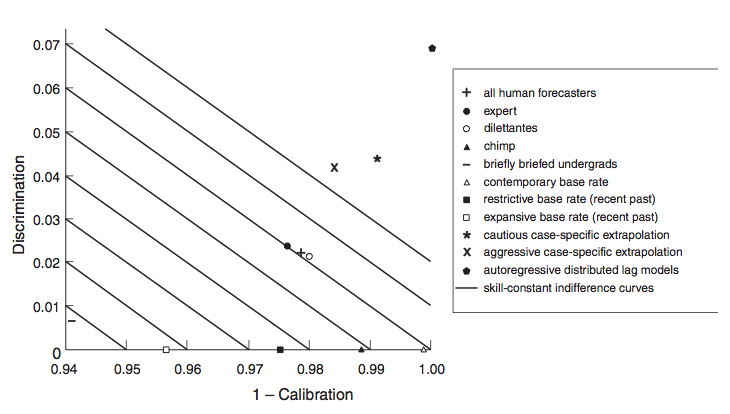
\includegraphics[width=\textwidth]{graphics/expert-political-judgment}

But, right, I'm getting a little carried away here. The point I'm trying to make
is that \textit{algorithms rule}. And, like I've argued before, everything can be
described as an algorithm. The entire scientific enterprise can be described as
algorithm-hunting.

The question, "How does the mind work?" is really looking for a step-by-step
process that the mind goes through to accomplish something -- when you can write
something down in such a way that a program can do, that's when you've
understood it.

If every process can be conceptualized as an algorithm, then, skills must fall
under that umbrella -- a skill is an algorithm, or as the quote at the intro
puts it, "A person taking a test or playing a piece of music is executing a
program, a deterministic procedure."

What are errors, then? Nothing but bugs in your program.

\section{Mistakes are valuable}

Humans are handicapped by our binary notion of correctness -- the notion that an
answer on a test is either correct or not. That there are no degrees.

But, after a bit of reflection, it becomes clear that one answer can be more
correct than another, while both can still be technically wrong.

Isaac Asimov has this to say on the subject in "The Relativity of Wrong,"

\begin{quote}
[W]hen people thought the earth was flat, they were wrong. When people thought
the earth was spherical, they were wrong. But if you think that thinking the
earth is spherical is just as wrong as thinking the earth is flat, then your
view is wronger than both of them put together.
\end{quote}
  
Once we abandon the binary notion of right and wrong, the actual nature of
wrongess becomes a bit more clear -- some of the haze dissipates. You will, if
you're paying attention, notice that wrongness is not one thing.

That there are many different ways to be wrong, and each of them have
indentifiable causes and the cause, once removed, eliminates the
wrongness. Thus, the label "stupid" or "bad at" are not so much explanations, as
they are frustrated noises that, when decoded, translate to "you're getting it
wrong but I don't understand the reason why."

When I was a student, I didn't understand this about wrongness and I didn't grok
that \textit{mistakes are evidence.}

Imagine you're a teacher, and you're grading 35 tests on, say, division,
and every test comes back the same: every student has answered that 100 divided
by 10 equals 90.

Are you going to say to yourself, "Well, I guess I just got a really dumb batch
of children this year. That's why they're getting it wrong."

No, of course not. You're going to go back over division with the children, with
an emphasis on the differences between division and subtraction -- because
apparently all the kids think you're asking them to subtract!

When you're learning something on your own, you have to be that teacher. If you
get something wrong, you need to stop, and pay attention to your mistake. With
mathematics, assuming you've kept reasonable notes, you can walk through your
answer, step by step, and see at which point you went wrong.

You can zero in on the bug and destroy it.

That's the process of debugging confusion.

\begin{itemize}
\item First, you get a problem wrong.
\item Then you must infer the cause of the mistake by collecting evidence.
\item Once you have the cause of the mistake, dispel the confusion, crush the bug,
  and update your programming.
\item Repeat this process until you've dispelled all of your bugs and reach the
  correct answer.
\end{itemize}

\section{Fixed versus growth mindsets}

\begin{quote}
  If you hear a voice within you say 'you cannot paint,' then by all means
  paint, and that voice will be silenced.
\end{quote}

Imagine, for a moment, that you are teleported to an alternate universe. The
year is 1891.

A 10 year-old boy named Pablo sits down in front of a piece of paper. He grips a
pencil in his right hand. On the table in front of him, an orange.

He closes one eye, concentrates on the orange, and moves the pencil across the
paper. He produces a line.

He looks at it, sighs, and gets up from the table.

The next day, the same thing happens. This goes on for weeks. Pablo's drawing of
an orange never improves. Always just a damned line.

\section{Dweck's research}

Carol Dweck has been doing research on what she calls fixed and growth
mindsets. The basic characteristic of a fixed mindset is believing that skills
and personality are not malleable -- they're fixed. You're either born good at
something or not, and that's the extent of it.

A growth mindset is the opposite: the belief that skill is something that can be
shaped through practice.

Dweck sometimes likes to present this in terms of intelligence, but I think this
is misleading. If you ask five people for a definition of intelligence, you will
get five different answers. That just confuses the issue.

Dweck should stop abusing lay notions of intelligence and just focus on skills.

As you may be anticipating, it's better for you to believe that skills aren't
fixed. Here, for instance, are the math grades of those who adopt a growth
versus a fixed view:

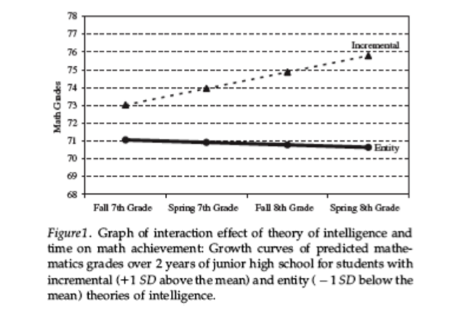
\includegraphics[width=\textwidth]{graphics/fixed-vs-growth-math-dweck}

And here's what happens when students are taught a growth mindset:

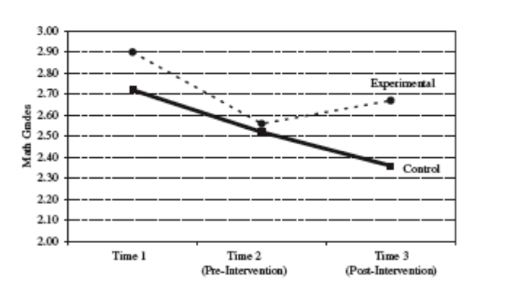
\includegraphics[width=\textwidth]{graphics/math-intervention-dweck}

Indeed, somewhat perversely, the fact that believing in a growth mindset
improves performance is evidence that a growth mindset is truer than a fixed
one: if believing you can do it improves your skills, it's hard to see in what
sense they're fixed.

And, indeed, that's the point of the Pablo parable. What would the world be like
if skills actually were fixed? No one would be able to whistle, Pablo Picasso
never would have drawn anything more than a line. Forget learning a second
language. Hell, forget learning a first language.

The point being: \textbf{Any skill can be improved with practice.}

\section{Paying attention}

Multi-tasking makes you stupid.

But don't take my word for it. Here it is from science's mouth:

\begin{quote}
Results show that when peripheral tasks interrupt the execution of primary
tasks, users require from 3\% to 27\% more time to complete the tasks, commit
twice the number of errors across tasks, experience from 31\% to 106\% more
annoyance, and experience twice the increase in anxiety than when those same
peripheral tasks are presented at the boundary between primary tasks.\cite{bailey2006need}
\end{quote}

I don't think you should ever be swayed by just one paper -- wait for the
replication.

But more than one paper finds that multitasking makes people stupid. Etienne
Koechlin and Sylvain Charron found, for instance, that increasing study
participants' tasks from 2 to 3 tripled error rates. \cite{charron2010divided}

There's a whole mountain of similar evidence, but I'm thoroughly convinced and
too lazy to dig up any more of it.

But wait, there's more.

One of the most exciting discoveries to come out of brain science during the
last century is the discovery that the brain is malleable, ``neuroplasticity.''
When you learn something new, this is reflected in structural changes to your
brain.

Or you know how Gary Busey seems a little off? This is because, in 1988, he
suffered a traumatic brain injury that resulted from a motorcycle accident --
indeed, one of the strongest arguments against the existence of a lasting, eternal soul
is that brain injuries can have such drastic and permanent affects on one's
personality.

Gary Busey is not a perfect example of neuroplasticity, though, because his
brain is different as a result outside forces (in his case, his head striking
the curb.) A better example?

Taxi drivers.

Katherine Woollett and Eleanor A. Maguire found, in a 2011 study that, when Taxi
drivers-in-training learned their way around London, this was accompanied by
measurable changes in the size of the posterior hippocampi -- a brain region
associated with spatial memory.

When you adapt, your brain adapts. When your brain adapts, you adapt. You are
your brain.

Why does this matter? Well, I'm going to tell you, and let me preface this with:
this is one of the most important things I've ever learned.

\textbf{Where you focus your attention controls which regions of your brain
  grow.}

This principle has been established first in monkeys, and since replicated
in humans several times.\cite{heron2010attention}\cite{stefan2004modulation} Here's how one of the studies\cite{recanzone1992topographic} went. Scientists trained owl
monkeys to hold their fingers on a ``tactile stimulator,'' which is a device like
this, that stimulates touch receptors. In order to receive a reward, the monkeys
had to pay attention to what their fingers were feeling.

As expected, the brain regions associated with touch grew.

Another group of monkeys had to undergo the same thing except, as you might
expect, they didn't need to pay attention to touch -- as a control, they had to
pay attention to an auditory task. The result? Little to no change in brain structures
associated with touch.

The paper itself puts it this way, ``The cortical representations of the trained
hands were substantially more complex in topographic detail than the
representations of unstimulated hands or of passively stimulated control
hands.'' In English, this says that larger, more complex brain regions were associated those monkeys who had
to pay attention.

I like to think of it this way: attention is the king of your brain and he's a
demanding king. Whenever something catches his interest, he starts yelling to
his people, ``Quick! Optimize my kingdom for my interests!''

So, concretely, if King Attention becomes interested in chess, he starts yelling
at the architects in his kingdom to start building chess libraries. He tells the
woodworks to get to work on giant chess pieces. The painters are forced to
paint giant chess boards on parking lots and to create chess themed art, and so
on.

Attention rules your brain, and he tells it what to build.

Here's the practical takeaway, then:

If you sit in front of the television with a textbook in front of you,
half-paying attention to both, you're going to triple your errors. Your brain
will become a little better at television watching, and a little better at the
subject associated with your textbook.

If you sit in front of a math problem, but pay more attention to your iPod than
to the problem, you'll get better at listening and understanding the
complexities of music. Pay attention to enough Beethoven and eventually you'll
be able to follow a fugue. Your math skills will go nowhere.

\textbf{To get better at anything, pay attention to it. Your brain will literally begin
reorganizing and optimizing itself for that task.} Focused attention is like
throwing fuel onto the fire that is skill acquisition.

\section{Deeper Processing}

\begin{quote}
  Most people would rather die than think; many do.
  \attrib{Bertrand Russel}
\end{quote}

The mind can be conceptualized as a network of connected links. That is, as a
graph, but not the sort that you learned about when you were taught how to plot
equations in the 7th grade.

No, a graph like this:

%tk picture of graph

So, thinking about the mind this way, here's the question that I have for you:
are you more likely to understand a concept if it's deeply entangled in your
neural web, connected to many different other concepts, or if you've just
connected it to one thing you know?

The first, of course and, indeed, there's some evidence to suggest that this is
true. It falls under the ``levels of processing effect.''

The basic theory: the more deeply that you process something, the more it
becomes entangled in your neural web, the better you'll understand and remember
it.

Here's how one study went. Scientists Craik and Tulving gave participants a list
of words. Some were asked to identify surface level features, things like
whether or not a word was italicized, or started with a certain letter. Other
participants were asked to think deeper about a word, like ``Can you meet
one on the street?''

Participants in the deeper processing group were able to remember more of the
words when later tested.

So, one way to ensure that you understand something is by attempting to connect
it to a number of things in your neural network, to consider it deeply. But how?

One of my favorite strategies is to consider \textit{why} something must be
so. If you learn a new fact, that's cool, and it's a good thing to know than to
not. But it's even better to understand why something is true. That is, to
understand why it necessarily follows from something else that you already know.

If you think about it, that's like connecting this new thing to old things that
you know.

But there's more to it than that. When you understand why something is true,
that knowledge can grow and change with you. You can apply it in different
circumstances, and you can understand when it applies and when it doesn't.

And, when you know why something works, you can modify it as you see fit --
like, now that you know that the principle here is to tightly connect a concept
inside of your neural web, you're not tied to mindlessly answering why
questions.

You can invent your own techniques.

Another possible reason why this technique works: it forces you to hold you
attention on something and, as you saw in the last section, focused attention
results in neural growth.

So maybe deep processing doesn't so much connect a concept to the rest of your
neurons, as it tricks you into focusing your attention onto it for a while.

In which case, you should invent techniques that help you hold your attention on
whatever skill it is that you want to master. I've heard a tennis technique:
just notice when the ball hits your racket, mentally say ``hit'', and when it
bounces on the ground, say ``bounce.''

Why is this effective? Because it focuses the mind on the game at hand. It
concentrates attention.

You don't necessarily need something complicated. Just noticing what you're
doing can be enough.

Oh, and one more technique when it comes to creating more mental connections:
when presented with a new concept, write down what it reminds you of. 

\section{Metaphor and Transfer}

During the first half of the 19th century, it was popular to teach Latin to
schoolchildren. Learning Latin was believed to teach rigor of mind. It taught
students how to think.

Today we know better -- sort of. Schools no longer bother teaching anyone but
historical scholars Latin, and we've abandoned the notion that Latin teaches
good thinking.

Unfortunately, this perennial idea, the notion that one subject can teach a mind
how to think, persists. Economists believe that economics teaches people how to
think. Mathematician think it about math. Computer scientists believe that, you
guessed it, computer science teaches that conveniently-head-to-measure
\textit{je ne sais quoi}: rigor of mind.

These are only the fields I'm familiar with. I'm sure game theorists believe it
about game theory, and maybe classical scholars believe that one cannot attain a
reasonable quality of thought without immersion in all of the great
metaphors. (An idea that used to have some appeal, given the number of colleges
that adopted teaching a ``Great Works'' program.)

Hell, there still exists a \textit{significant} amount of the population that
believe chess skill reflects something other than
amount-of-time-spent-playing-chess. I've heard from a guy who picked up chess in
order to improve his mathematical ability.

I doubt all of these claims. One of the most troubling findings to come out of
modern educational psychology has been that the transfer of learning is a sort
of popular myth -- it happens, but it's far from normal.

Instead, when people are taught one thing, well, they learn that one,
hyper-specific lesson. An algebra class won't teach students algebra -- it will
teach students how to solve algebra problems when given an algebra book. It
emphatically won't teach students to realize ``Hey, I can use this to solve
actual problems that I have.''

Or, you know, the entire reason that algebra was invented in the first place.

Douglas Detterman puts it this way, ``In general, I subscribe to the principle
that you should teach people exactly what you want them to learn in a situation
as close as possible to the one in which the learning will be applied.  I don't
count on transfer and I don't try to promote it except by explicitly pointing
out where taught skills may be applied.''

Which brings me to my point: don't plan on knowledge transferring. Instead,
train in the way that you want to be able to perform. The closer you can get the
two conditions, the better.

Still, this is a little hard to swallow.  When it comes to each new skill, I'd
rather not start from zero.

I'd like to instead use what I already know to leap forward, to become better
than someone with no other knowledge.

In short, I'd like to build some kind of bridge between one skill and another,
supercharging my performance at that new school.

What do you call a bridge between old knowledge and new? One that lets you use
old knowledge as if it, too, applied in this new situation, such that you don't
need to learn everything all over again?

A metaphor. You want a metaphor.

\section{Analogical Thinking}

\begin{quote}
Analogy is our best guide in all philosophical investigations; and all
discoveries, which were not made by mere accident, have been made by the
help of it. \label{quote-attribute}{---Joseph Priestley}
\end{quote}

Words are not the stuff of thought.

This is straightforward to demonstrate. Present someone with a quote --
it can be anything, but for concreteness let's say you go with a bit of
Thoreau: ``I was not designed to be forced. I will breathe after my own
fashion. Let us see who is the strongest.''

So, you present this line to someone, and then you let some time pass,
say an hour. Then, ask them to repeat the quote back to you. What do
they tell you?

I'd wager that you don't get the exact quote back, but the gist of the
thing. Sort of like when reading this, you will come away not with an
exact memory of each word and every comma, but instead a general idea of
what it is that I'm talking about -- a summary. Almost as if your mind
were a lossy compression algorithm.

If words were the stuff of thought, or at least of memory, you'd expect
the mind to store words as, well, words. If words were the stuff of
thought, when presented with a quote, on recall you'd repeat the exact
quote back.

But, instead, there seems to be some kind of mental translation that
goes on. You don't remember the exact quote but, instead, it gets stored
as a ``gist,'' as if your mind translated it to meaningness.

So, words are not the stuff of thought.

Let me put it another way. What I'm saying is that, \textbf{when you are
offered some concept in words, you store that concept in meaning-nese.
And, then, when you communicate it with someone, you translate that
meaning-nese back into words.}

This explains why the quotes are not exact, but become garbled -- the
words have to undergo translation: first, from words to meaning-nese to
be stored, and then from meaning-nese back into words during recall.
It's like taking English, translating it into Chinese, and then
translating it back into English.

You won't end up with the original English.

\subsection{How this relates to
metaphor}\label{how-this-relates-to-metaphor}

\begin{quote}
Analogy is anything but a bitty blip --- rather, it's the very blue that
fills the whole sky of cognition --- analogy is everything, or very
nearly so, in my view. \label{quote-attribute}{---Doug Hofstadter}
\end{quote}

Now, with this in mind, let's consider the problem of communication. To
make this easier, let's restrict ourselves to idealized communication --
comminucation where the goal really is communication. This is different
from communication ``in the wild'', where a lot of talking is not about
substance, but about expressing friendliness or (perhaps unconsciously!)
furthering one's agenda.

So, idealized communication, where discussion really is about the
transfer of ideas. Given this idea of meaningness translation, what can
we say about this transfer?

Well, the goal of communication is for the speaker to translate some
useful structure she has in her mind, encoded in meaning-nese, and to
re-encode it in some other form -- typically language, but it could also
be art, or movement, whatever.

Then, the task of the listener, is to take this language-encoded
structure and to decode it back into the original meaning-nese -- or, at
least, some dialect of meaning-nese compatible with the listener's mind.

Thus, \textbf{communication is really about the transfer of useful mind
structures between speakers -- but, since we can't directly transfer
from one brain to another via an uplink ala \emph{The Matrix}, there's
an intermediate encoding and decoding step.}

Visually:

\begin{figure}[htbp]
\centering
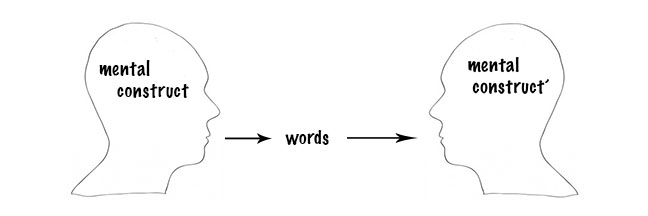
\includegraphics[width=\textwidth]{graphics/analogical-thinking.jpg}
\caption{Picture of a concept moving from mental construct, mapped into
words, and then back to mental construct, to illustrate analogical
thinking.}
\end{figure}

\subsection{What labels imply}\label{what-labels-imply}

Okay, let's take a step back then and consider the implications. What
does it mean when you encounter a word or a phrase that you don't
understand? What does that indicate?

If we take the encode-decode dance literally, it's an indication that
the speaker has some useful cognitive structure in her head, with which
you're unfamiliar. So, concretely, I recently learned the word
``ostensibly'' which means ``as it seems on the surface, but perhaps not
actually.''

I have found this a gratifying label to have in my head, now that I've
gone through the effort of re-building the cognitive structure that it
represents. I can say something like, ``Big business is ostensibly
pro-immigration reform because they care about the welfare of would-be
immigrants.'' And ``ostensibly'' here acts as a sort of wink that says,
yeah, that's one explanation, but maybe there's something more to it. In
this example, this something more would be that maybe business just
cares about cheap labor.

So, what am I trying to say here? What's the practical interpretation?
When you come across some equation, word, phrase, or whatever, that
strikes you as foreign, \textbf{this signals that the person has some
useful cognitive structure that you don't.}

\subsection{What does this have to do with
analogy}\label{what-does-this-have-to-do-with-analogy}

Now, in a section that is about analogical thinking, you are maybe
wondering why I've taken you through this detour into communication and
cognitive structures. The idea is that, in some sense, all language acts
as a metaphor.

This notion has recently been making the rounds with the endorsement of
Doug Hofstadter, of
\href{http://www.amazon.com/gp/product/0465026567/ref=as_li_tl?ie=UTF8\&camp=1789\&creative=390957\&creativeASIN=0465026567\&linkCode=as2\&tag=rsio-20}{\emph{Gödel,
Escher, Bach}} (very recommended) fame, but the idea is at least as old
as Lakoff and Johnson's
\href{http://www.amazon.com/gp/product/0226468011/ref=as_li_tl?ie=UTF8\&camp=1789\&creative=390957\&creativeASIN=0226468011\&linkCode=as2\&tag=rsio-20}{\emph{Metaphors
We Live By}} (and, no doubt, older still than that.)

Here is what I mean when I say that all communication is analogy.
Consider again the encode-decode theory I just told you about: it's
about taking meaning-nese, mapping it into words, and then unmapping it
back into meaning-nese.

What do you call a mapping between two different things? An analogy. So,
in a sense, \textbf{all communication is about constructing an analogy
between cognitive structures and words, and then the task of the
listeners is to decode that analogy into their own mental model.}

Essentially, that's what's happening right now: I'm encoding my ideas
here, as words, and you, the reader, are decoding them. And, if
everything is going as planned, you're building a cognitive structure in
your head right now which is similar to the one that I have in mind.

This is what separates a good exposition from a bad one: with a good
one, it's easy to decode and build up the writer's cognitive structures
in your own mind. With bad exposition, you either end up with no
structure or a damaged one, a misunderstanding.

\subsection{Concepts as analogical
  bundles}\label{concepts-as-analogical-bundles}

\begin{quote}
A good stack of examples, as large as possible, is indispensable for a thorough
understanding of any concept, and when I want to learn something new, I make it
my first job to build one.
\attrib{Paul Halmos}
\end{quote}

In fact, we can go even a little further than this, and say, what is a
concept, \emph{really}? That is, what are these cognitive structures
that I have in my mind?

As a concrete example, let's consider the number three. What is the idea
of three-ness?

Well, with the concept, if you wanted to transfer it to a young child,
you'd give concrete examples. A group of three rocks, three bananas, and
so on, except of course you wouldn't say ``three'' -- you would show
them three rocks, three bananas, and you'd ask them, so, what do these
things have in common?

With enough examples, they would catch on, or at least so I suspect.
I've been unable to acquire the necessary funding to experiment on young
children.

The idea, though, is that with any concept, when you start unbundling
it, you find that it's really just a bunch of examples with some common
core -- some hidden structure, that isn't immediately obvious when you
consider just one thing in isolation, but becomes apparent with the
study of tangible examples.

That is, \textbf{a concept is a bundle of examples.} The process of
abstraction, of obtaining a useful cognitive structure, is ultimately
one of comparing and contrasting these examples, until have built up
this structure in your mind.

\subsection{Some evidence regarding analogical
  thinking}\label{some-evidence-regarding-analogical-thinking}

\begin{quote}
I had a scheme, which I still use today when somebody is explaining something
that I'm trying to understand: I keep making up examples.
\attrib{Richard Feynman}
\end{quote}

So, let's recap for a moment:

\begin{itemize}
\itemsep1pt\parskip0pt\parsep0pt
\item
  Communication is the process of translating a cognitive structure into
  words, and then from words back into a cognitive structure.
\item
  This mapping and unmapping is an analogy: setting up an isomorphism
  between cognitive structures and words.
\item
  A concept is a bundle of concrete examples. Each example contains some
  common core, with is captured in the concept. Thus, every concept is
  itself an analogy.
\end{itemize}

So, really, here we have two different uses of analogy: a
concept/cognitive structure is an analogy, and we use a process of
analogy to transfer them between people.

If this is really true, if I'm not just spinning you a nice story, we
ought to expect that the study of concrete examples is the best way to
go about learning a new concept. Really, it's probably the only way to
build a new cognitive castle in your head.

Is there any evidence to support this view? Well, yes. There's
\href{http://psycnet.apa.org/journals/edu/95/2/393/}{significant
evidence} suggesting that \textbf{comparing and contrasting examples is
a powerful technique when it comes to understanding something new.}

Consider the inert knowledge problem. This is when you're in a
situation, and you have relevant, applicable knowledge, but you fail to
apply that knowledge. So, concretely, say you've taken a basic calculus
class, and you're arguing with someone about population growth. You get
in this heated disagreement. They say that our current growth is
unsustainable, and we're headed towards an inevitable collapse because
there is not enough food to go around -- a Malthusian catastrophe.

You take a contrary position, and point out that, as nations develop,
birth rates fall, such that population growth is below the replacement
rate in some developed nations, like Japan and Germany. At a certain
tipping point of prospertiy, population plateaus and then actually
begins to fall.

If your calculus knowledge transferred, here you might realize that this
is an argument about the shape of the derivative of population growth.
And, if you so realized, you might both draw out curves of what you
think it looks like, and then compare that to real-world data.

The inert knowledge problem would be 1) knowing calculus, 2) having this
argument, and 3) not realizing that you're actually arguing about
derivatives.

Now, depending on the amount of learning you've done in the past, you
may or may not have noticed that inert knowledge is the devil. Why learn
something if you fail to apply it? What can be done about this?

Well, okay, learning something is about the acquisition of concepts,
right? So calculus knowledge is about building up calculus structures in
your head.

If, as I've argued, this is the case, we might expect that comparing and
contrasting examples (and thusly promoting concept acquisition) would
help us overcome the inert knowledge problem.

Is this the case?

Yes. \textbf{There's even some evidence that comparing and contrasting
examples, ``analogical encoding'', is potentially the only effective
technique at dealing with this inert knowledge plague.} One review
\href{http://onlinelibrary.wiley.com/doi/10.1111/j.1551-6709.2009.01070.x/full}{put
it this way}: ``The best-established way of promoting relational
transfer is for the learner to compare analogous examples during
learning (Catrambone \& Holyoak, 1989; Gentner, Loewenstein, \&
Thompson, 2003; Gick \& Holyoak, 1983; Reeves \& Weisberg, 1994; Ross \&
Kennedy, 1990; Seifert et al., 1986, Experiments 1 and 2).''

The quoted study further finds that analogical encoding -- comparing and
contrasting examples -- not only promotes future transfer, but actually
works backwards, too.

What do I mean by this? I mean that, if you sit down and compare and
contrast examples, you're going to be much more effective at coming up
with past, relevant experiences of the principle in question. You can
use this to transform inert knowledge into animated knowledge. To piece
together the once dead into a new Frankenstein's monster.

To use our calculus example again, if you're reading about the jerk (the
rate of change in acceleration), and you compare and contrast real-world
examples, you're more likely to spontaneously realize that, when
learning to drive, the jerk you felt when stopping too quickly was an
example of, you know, the jerk in physics.

\subsection{Benefits for the acquistion of
expertise}\label{benefits-for-the-acquistion-of-expertise}

So, at this point, I hope you're convinced that comparing and
contrasting examples is \emph{the} way to go about acquiring a new
concept -- it's how to absorb a bundle of concrete examples and distill
them into a useful cognitive structure.

But that's not all! This is not the only benefit. Consider what it means
to be an expert at something. One of
\href{http://eric.ed.gov/?id=ED215899}{the most cited studies on
expertise} compared how graduate students in physics categorized physics
problems, versus how novices did.

The finding? Physics experts were more likely to pick out the underlying
physical principle, while novices tended to focus on irrelevant surface
characteristics. Presumably, physics experts had built up a cognitive
structure that they recognized in the problem. The novices, lacking this
mental structure, were unable to spot it.

If the theory I have sketched here is correct, then we ought to expect
that \textbf{comparing and contrasting examples will accelerate the
acquisition of concepts and therefore expertise}. Analogical encoding
allows one to swim out from shallow seas and into the depths --
``\href{http://onlinelibrary.wiley.com/doi/10.1111/j.1551-6709.2009.01070.x/full}{comparison
between two analogous examples acts to make their common relational
structure more salient} (Gentner \& Medina, 1998; Gentner \& Namy, 1999;
Markman \& Gentner, 1993).''

\subsection{Practical implications}\label{practical-implications}

Okay, then, we've just breezed through the core ideas of analogical
thinking. To sum it up:

\begin{itemize}
\itemsep1pt\parskip0pt\parsep0pt
\item
  Words are not the stuff of thought. Our minds translate words into
  something else (meaning-nese).
\item
  Communication is essentially about analogy: it's about mapping a
  cognitive structure (``meaning-nese'') into words, and then the
  listener unpacks that back into a cognitive structure.
\item
  Thus, sucessful communication is about setting up understandable
  analogies.
\end{itemize}

Then, I covered the relationship between concepts and analogy:

\begin{itemize}
\itemsep1pt\parskip0pt\parsep0pt
\item
  A concept is a bundle of concrete examples that illustrate some core
  relationship between those examples. The concept of three-ness can be
  understood as the relation between concrete instances of three things
  (bananas, rocks, years).
\item
  Given that a concept is a bundle of examples, we should expect that
  the best way to acquire a useful cognitive structure is to compare and
  contrast examples (``analogical encoding'').
\item
  There is a significant body of evidence that suggests that this is the
  case: comparing and contrasting examples is a powerful way to acquire
  a concept.
\end{itemize}

I also touched on the inert knowledge problem, and how analogical
encoding allows us to overcome it:

\begin{itemize}
\itemsep1pt\parskip0pt\parsep0pt
\item
  The inert knowledge problem is when you have relevant knowledge but
  fail to take advantage of it. Example: failing to realize that an
  argument about population growth is an argument about the shape of a
  derivative.
\item
  The only consistely supported method of overcoming the inert knowledge
  problem, and promoting the application of a concept in new situations
  (``transfer''), is analogical encoding -- by comparing and contrasting
  examples. ``When subjects explicitly compared the analogs and then
  immediately attempted to solve the target problem in the context of a
  single experiment, transfer was obtained with significant frequency
  even without a hint that the analogs and target were related. (Holyoak
  and Catrambone)''
\end{itemize}

Finally, I mentioned how this relates to expertise:

\begin{itemize}
\itemsep1pt\parskip0pt\parsep0pt
\item
  Experts are distinguished by better developed cognitive structures.
  Physics experts, for example, are able to pick up on the underlying
  structure of physics problem, while novices focus on sufrace
  characteristics.
\item
  How can we acquire such a cognitive structure? By analogical encoding
  -- comparing and contrasting examples. Contrasting examples fosters a
  focus on deeper structures.
\item
  Thus, to accelerate the acquisition of expertise, one should take
  advantage of analogical encoding.
\end{itemize}

So, practically speaking, how can you, as an individual put this into
practice? This method, analogical encoding, is both simple and powerful.
\textbf{To acquire a new cognitive structure, gather together a bunch of
examples of the concept, and then compare and contrast those examples.}

If you would like to improve your calculus skill, you should Google for
real-world examples of derivatives or integrals or any concept that
you'd like to acquire. Then, write them down, and then list how each is
similar and each is different.

You can also use these principles to improve your communication and
teaching skills. If you want someone to obtain a cognitive structure
that you have, illustrate the principle with examples, and then bring
their attention to the underlying similarity connecting the examples. In
the case of this section, the principle behind all of these examples has
been that learning and communication is about the transfer of concepts,
which are bundles of examples, and can be acquired by contrasting
concrete examples.

Now, what was that Thoreau quote, again?

\subsection{Further Reading}\label{further-reading}

\begin{itemize}
\itemsep1pt\parskip0pt\parsep0pt
\item
  If you enjoyed this, check out a copy of
  \href{http://www.amazon.com/gp/product/0226468011/ref=as_li_tl?ie=UTF8\&camp=1789\&creative=390957\&creativeASIN=0226468011\&linkCode=as2\&tag=rsio-20}{\emph{Metaphors
  We Live By}},
  \href{http://www.amazon.com/gp/product/B00BE65086/ref=as_li_tl?ie=UTF8\&camp=1789\&creative=390957\&creativeASIN=B00BE65086\&linkCode=as2\&tag=rsio-20}{\emph{Surfaces
  and Essences}}, or
  \href{http://worrydream.com/refs/Hofstadter\%20-\%20Analogy\%20as\%20the\%20Core\%20of\%20Cognition.pdf}{``Analogy
  as the core of cognition.''}
\item
  This is far from the first time that I've written about learning and
  expertise. Check out my articles on
  \href{http://rs.io/2014/02/21/problem-solving.html}{the science of
  problem solving},
  \href{http://rs.io/2014/02/25/why-questions-reveal-structure.html}{the
  importance of ``why?'' questions},
  \href{http://rs.io/2014/02/24/compressing-knowledge.html}{compressing
  knowledge}, and the
  \href{http://rs.io/2014/01/20/human-expertise-and-memory-machines.html}{role
  of memory in human expertise}. Oh, and if you just want to enjoy a
  metaphor, none of mine have resonated more with the internet at large
  than
  \href{http://rs.io/2014/02/26/why-online-communities-decay-over-time.html}{online
  communities as vampire bat colonies}.
\end{itemize}

\section{Teaching others}

Let's say, for the sake of discussion, that you, the gentle reader, are
a good, virtuous human being. And this implies that, as a good, virtuous
human being, you don't stock up on trashy, vampire-themed romance novels
or the male-equivalent, science fiction and horror. (Two genres to which
I owe a troubling portion of my youth. Science fiction and horror, that
is. Not vampire romance. Okay, maybe a little vampire romance.)

No. As a kind and decent reader, you consume a steady diet of textbooks.

So, being fair, humble, textbook reading folk, you have a dilemma:
what's the best way to maximize the amount of knowledge that you suck
out of something that you read? How can you, like the proverbial
vampire, drain your victim and thusly replenish your own life-essence?

Let's say I narrow the search space down for you. Which is going to have
better results?

\begin{itemize}
\itemsep1pt\parskip0pt\parsep0pt
\item
  Reading with the aim of maximizing your own personal knowledge, like
  you might to pass a test.
\item
  Reading with the goal of teaching the material to someone else.
\end{itemize}

You can probably guess that the second option is the one I want to talk
about -- not because you know that's going to be the answer, but because
you have a heuristic that goes something like, ``The author doesn't tell
me obvious things that everyone already knows.'' So don't get too cocky
here, buddy. If I'd started this section with, ``The best way to learn
something is to pretend that you're going to have to pass a test on it
in the future,'' you'd have swallowed that like a big dumb fish.

So, concretely, when you go to learn something, learn with the intention
of teaching it to someone else. This doesn't have to be a real person,
or a person at all. You'll reap almost all of the benefits by learning,
say, the capital asset pricing model with the intention of teaching it
to your dog. I mean, dogs are at least more interactive than rubber
ducks, and I guess you can interpret barks as, ``Explain, please. I'm
lost.''

An actual person is better still -- this is one of the main motivations
for my writing. It's an exercise in clarifying and solidfying my own
thoughts, and as a pretty excellent bonus, I also create something of
value.

In fact, one study even found participants who read something and then
taught it to others outperformed those who read something and then went
over it with a tutor.

Let that sink in for a moment. You know how everyone is paying many
thousands of dollars a year to go to a college, at least some of them to
``get an education''? Yeah, you, right here and now, could better master
the same material by checking out a textbook from the library, reading a
chapter, and then trying to teach it to anyone you can convince to
listen.

For a cost of zero.

Let me put this another way: at the time of this writing, the median
cost for one year of college is about 15 thousand dollars, and most
students are taking 5 or more years to graduate, for a price tag (not
counting opportunity costs) of more than 75,000 dollars. I've just
taught you a simple, portable method that will achieve better cognitive
results (assuming a sufficiently motivated reader), and can be
implemented for the cost of a library card.

Even if we are very cynical and say that the education part of college
is only 2\% of the value of a degree, that piece of info I just gave you
is still worth 1500 dollars.

So, I guess what I'm saying is: you're welcome.

\subsection{The Feynman method}\label{the-feynman-method}

Scott Young has a technique that captures this nicely, which he's dubbed
``the Feynman technique.'' This is better than what I came up with:
the-harass-your-girlfriend-into-listening-to-you-talk-about-the-Fama--French-three-factor-model-technique.
A mouthful, to be sure.

Here's how it works: 1. Read a chapter (or watch a video, etc). 2. Write
down an explanation, like you're explaining it to someone else. (I
typically like to use past-me as a model.) 3. When you're uncertain
about something, go back to the textbook.

This techinque, my friend, is a thing of beauty. It has strong empirical
support: I've just mentioned research that says teaching someone leads
to greater learning and, as you're about to see, the art of memory is
really the art of recall.

Keep reading.

\subsection{Putting it all together}\label{putting-it-all-together}

For when you inevitably forget everything that I wrote in this chapter,
here is a condensed version of the major points.

\begin{itemize}
\itemsep1pt\parskip0pt\parsep0pt
\item
  To understand the core of something, collect many different
  perspectives. Read more than one recipe for the same dish, and more
  than one textbook on the same subject.
\item
  Your mistakes are valuable information. You have a bug somewhere. What
  is it?
\item
  To take your performance now from incorrect to correct, identify the
  problems in that performance (bugs) and fix them.
\item
  There are no such things as fixed skills. Anything you'd like to
  better at, you can be better at, with practice.
\item
  What you pay attention to physically determines which regions of your
  brain grow and change. Thus, if you want to understand or be better at
  something, pay close attention to it. Attention is the king of your
  brain and he's a demanding king. Whenever something catches his
  interest, he starts yelling to his people, ``Quick! Optimize my
  kingdom for my interests!''
\item
  To get a deeper understanding of something, focus on why it's true.
\item
  Communication is ultimately a process of analogy: making words and
  symbols on paper into cognitive structures.
\item
  Concepts are bundles of conrete examples that have something in
  common.
\item
  To understand something really, to get at the core of it, compare and
  contrast examples. This will boost understanding and improve the
  flexibility of your knowledge, so that you'll be more likely to apply
  it in the future.
\item
  Comparing and contrasting examples (``analogical encoding'') may also
  accelerate the acquisition of expertise.
\item
  When you learn, learn with the aim of teaching the subject matter to
  someone else. This is more effective than someone else teaching the
  subject to you.
\item
  To take advantage of this, use the Feynman technique: read something,
  then write it down like you're explaining it to someone else. When you
  become stuck or confused, go back to the book.
\end{itemize}

The reader who takes advantage of one, two, or three of these techniques
persistently can expect to reap significant gains in learning ability.
When combined with a strong research ability and understanding of
memory, you can expect much more. But you'll have to read the next
chapter for that.
